% !TeX encoding = UTF-8
%



\section{Screenshots}
\label{Anhang:Aufnahmen}


~\\



\newpage



% % % % Test-Bau-Knoten % % % %

\subsection{Testknoten}

Ein Bilderkatalog der die Knoten zeigt, deren Erstellbarkeit wir explizit prüfen. Hinweis: Mit Adobe Reader ab Version 9 ist es möglich den Knoten-Bau als Animation abzuspielen.\\


	\subsubsection*{\glqq {"U}berleger\grqq}
	
	% TODO: Störende Vorschau umgehen.
		\begin{figure}[!h]
		
			\label{Abb:Test-Knoten:Ueberleger}
			\centering	
			
			\includemedia[activate=onclick]
			{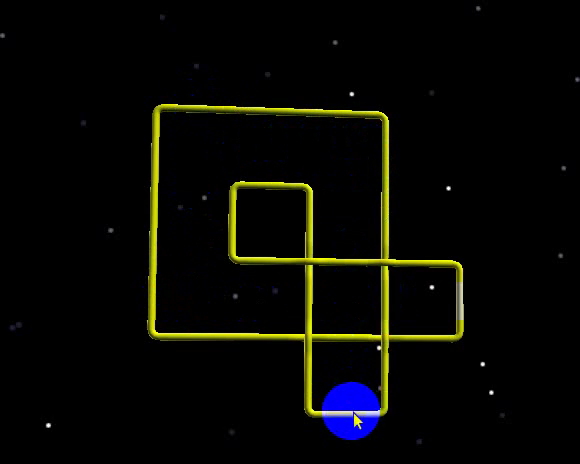
\includegraphics[width=\textwidth]
			{\testknots/Ueberleger/Ueberleger.png}}
			{\testknots/Ueberleger/Ueberleger.swf}
			
		\end{figure}
		
		~\\\mousecursor~\hyperref[FT:30:Ueberleger]{Siehe Funktionstest FT\_30.} 
	
	
\clearpage	


	\subsubsection*{\glqq Schlaufe\grqq}	
	
		\begin{figure}[!h]
		
			\label{Abb:Test-Knoten:Schlaufe}
			\centering	
			
			\includemedia[activate=onclick]
			{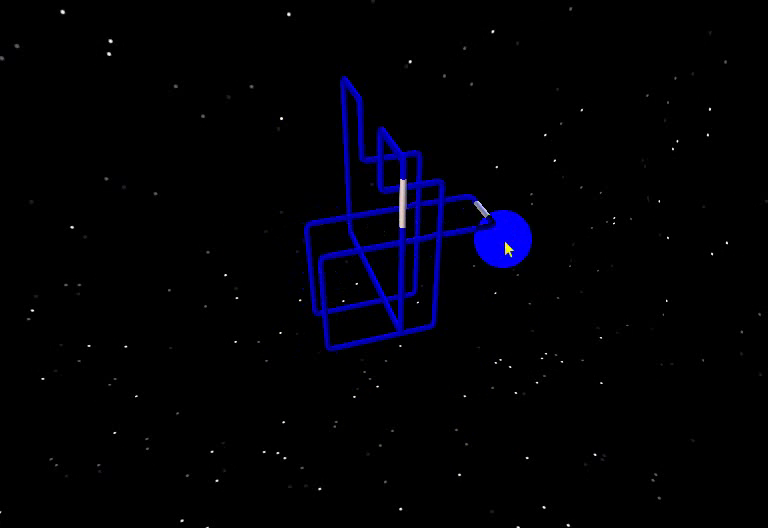
\includegraphics[width=\textwidth]
			{\testknots/Schlaufe/Schlaufe.png}}
			{\testknots/Schlaufe/Schlaufe.swf}
			
		\end{figure}
		
		~\\\mousecursor~\hyperref[FT:30:Schlaufe]{Siehe Funktionstest FT\_30.} 
	
	
\clearpage	
% 



\newpage



% % % % Grafikfehler % % % %

\subsection*{Grafikfehler}



\newpage



\subsection*{Werkzeuge}


% Code-Coverage Report Build-Script

\begin{figure}[ht]

	\centering
	%\label{Abb:Werkzeuge:Code-Coverage_Build-Script}
	
	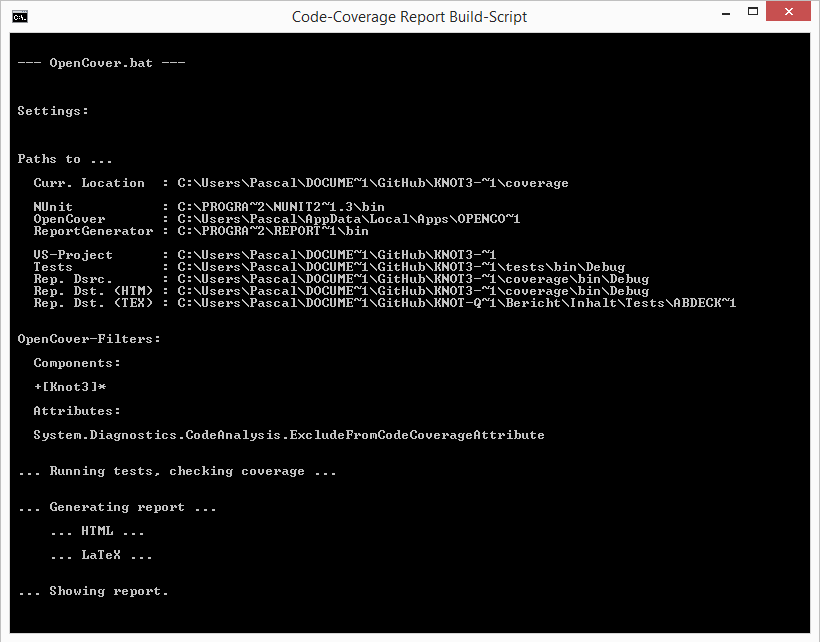
\includegraphics[width=\textwidth]{Inhalt/Anhang/Grafiken/Werkzeuge/Code-Coverage Report Build-Script.png}
	
	\caption{Build-Batch für die Erstellung des Testabdeckungs-Berichts.}

\end{figure}








